\documentclass{beamer}
\usepackage[english]{babel}
\usepackage{amsmath,graphicx,hyperref}

%%%%%%%%%% Start TeXmacs macros
\newcommand{\cdummy}{\cdot}
\newcommand{\mathd}{\mathrm{d}}
\newcommand{\nospace}{}
\newcommand{\tmmathbf}[1]{\ensuremath{\boldsymbol{#1}}}
\newcommand{\tmop}[1]{\ensuremath{\operatorname{#1}}}
\newcommand{\tmstrong}[1]{\textbf{#1}}
%%%%%%%%%% End TeXmacs macros

\begin{document}

{\screens{{\screens{\begin{frame}
  \
  
  \
  
  \
  
  \
  
  \
  
  \title{计算视觉与模式识别}
  
  \maketitle
  
  \ 
\end{frame}}{\begin{frame}
  \
  
  \resizebox{1\columnwidth}{!}{\includegraphics{img/sun_image.png}}
\end{frame}}{\begin{frame}
  {\hspace{3em}}\resizebox{0.8\columnwidth}{!}{\includegraphics{img/camera-image-1.png}}
\end{frame}}{\

{\hspace{3em}}\resizebox{280pt}{!}{\includegraphics{img/Camera-Obscura.jpg}}}{\begin{frame}
  \frametitle{照相机与摄像机}
  
  {\hspace{6em}}\resizebox{0.6\columnwidth}{!}{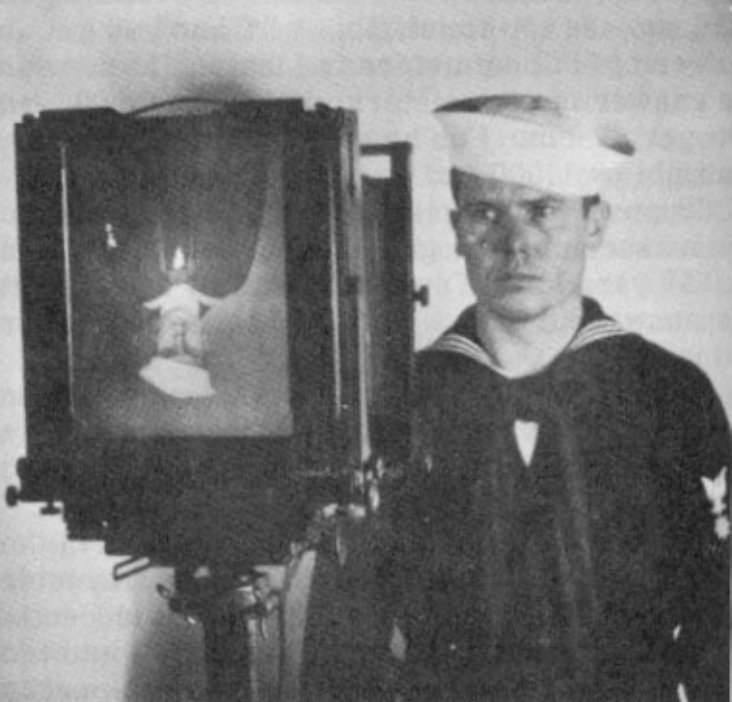
\includegraphics{img/sailor.png}}
\end{frame}}{\begin{frame}
  \frametitle{针孔相机}
  
  \label{attachment_494307}\qquad\resizebox{0.9\columnwidth}{!}{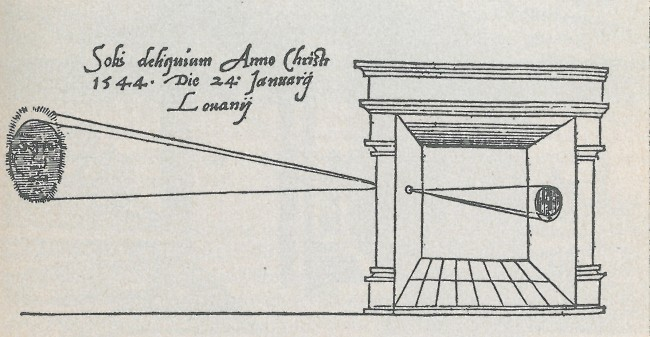
\includegraphics{img/cameria-obscura-illustration-2.jpg}}
  
  \label{caption-attachment-494307}First published illustration of camera
  obscura in Gemma Frisius' book ``De Radio Astronomica et Geometrica,'' 1545
  (Photo:
  \href{https://commons.wikimedia.org/wiki/File:1545_gemma_frisius_-_camera-obscura-sonnenfinsternis_1545-650x337.jpg}{Wikimedia
  Commons}, Public domain)https://mymodernmet.com/camera-obscura/
\end{frame}}{\begin{frame}
  \frametitle{透视投影}
  
  \
  
  \
  
  {\hspace{3em}}\resizebox{0.8\columnwidth}{!}{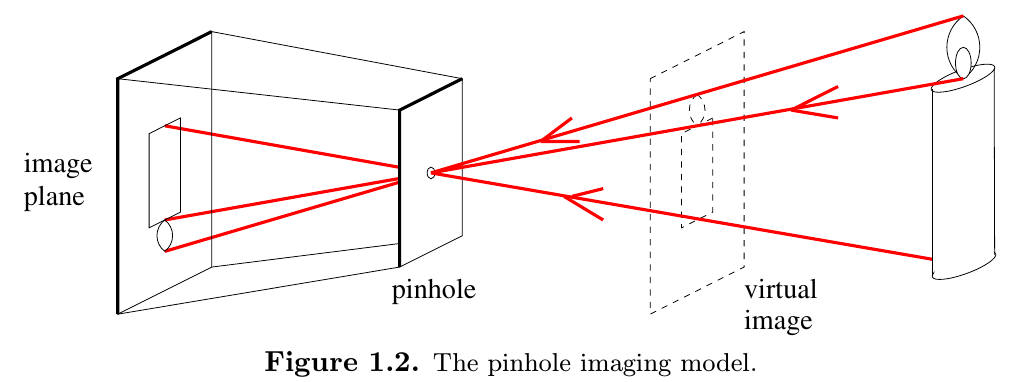
\includegraphics{img/pinhole_imaging.png}}
  \begin{eqnarray*}
    &  & 
  \end{eqnarray*}
\end{frame}}{\begin{frame}
  \frametitle{}
  
  \
  
  {\hspace{3em}}\resizebox{0.8\columnwidth}{!}{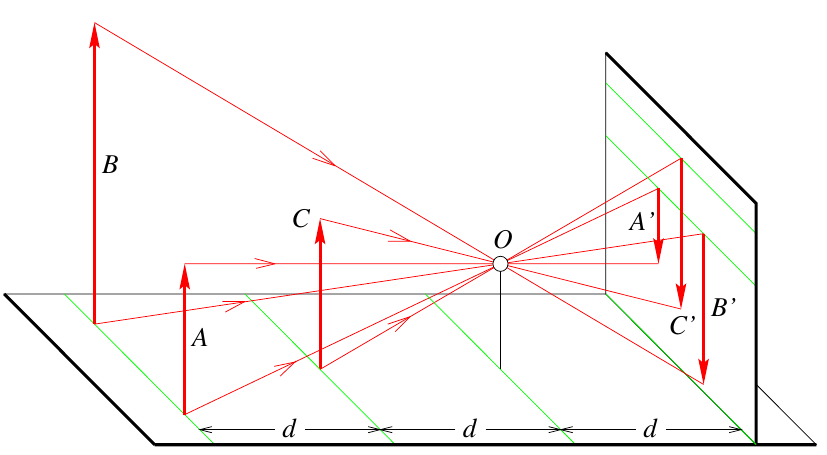
\includegraphics{img/perspective_effects.png}}
\end{frame}}{\begin{frame}
  \frametitle{}
  
  \
  
  \
  
  \qquad\resizebox{0.8\columnwidth}{!}{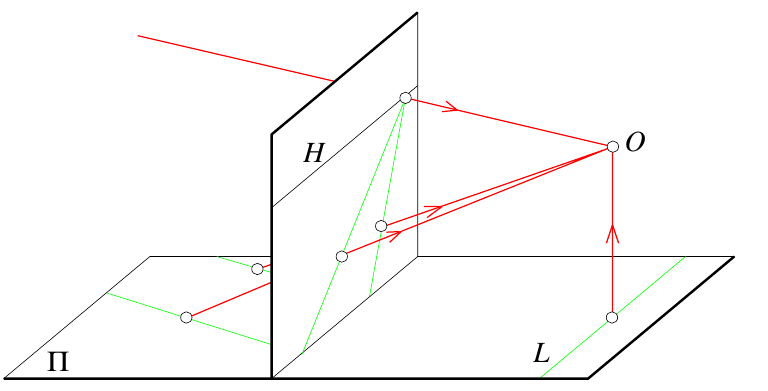
\includegraphics{img/parallel_lines_converge.png}}
\end{frame}}{\begin{frame}
  \frametitle{}
  
  \
  
  \
  
  \resizebox{1\columnwidth}{!}{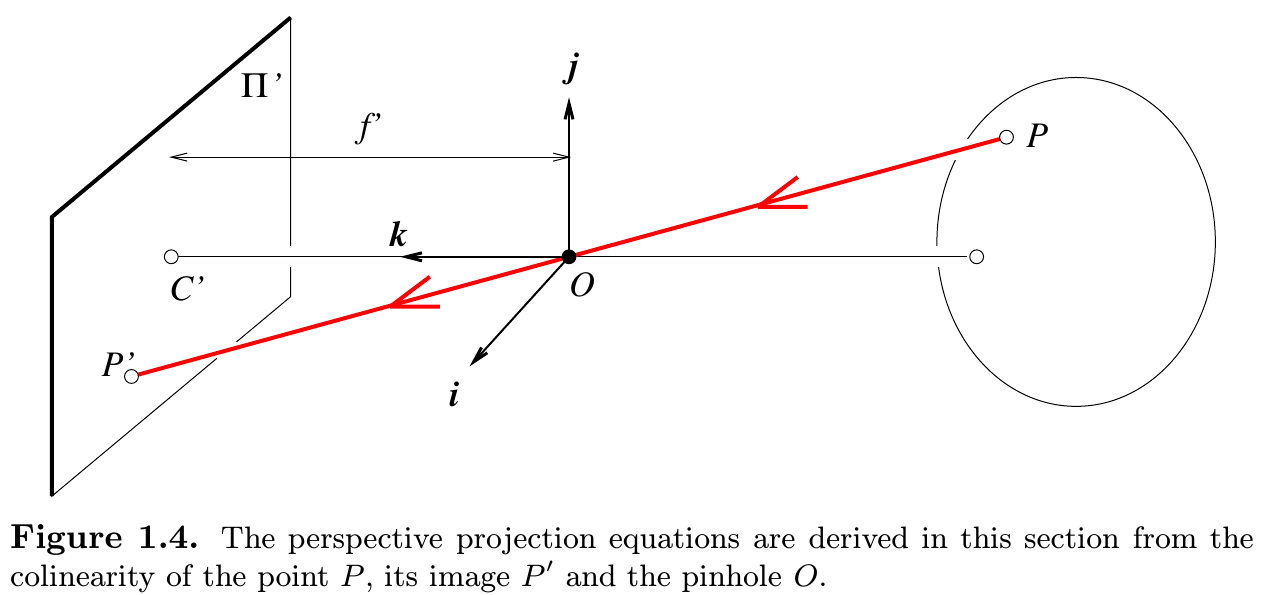
\includegraphics{img/perspective_projection.png}}
  
  \ 
\end{frame}}{\begin{frame}
  \frametitle{透视投影模型}
  
  
  \begin{eqnarray*}
    \left(\begin{array}{c}
      x'\\
      y'\\
      f'
    \end{array}\right) & = & \lambda \left(\begin{array}{c}
      x\\
      y\\
      z
    \end{array}\right)
  \end{eqnarray*}
  \[ \lambda = \frac{x'}{x} = \frac{y'}{y} = \frac{f'}{z} \]
  therefore
  \begin{eqnarray*}
    x' & = & f' \frac{x'}{z}\\
    y' & = & f' \frac{y'}{z}
  \end{eqnarray*}
  
\end{frame}}{\begin{frame}
  \frametitle{弱透视投影}
  
  \
  
  \
  
  \qquad\resizebox{0.8\columnwidth}{!}{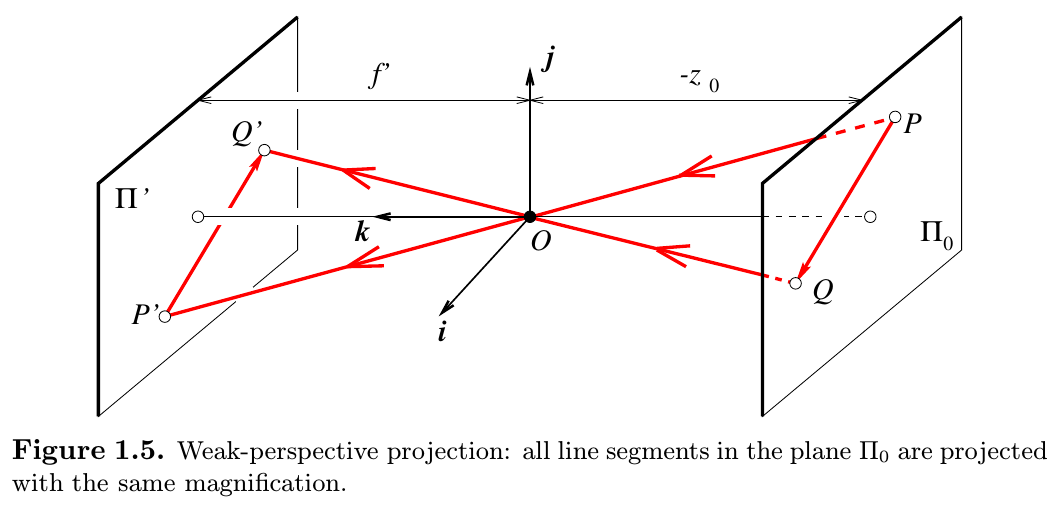
\includegraphics{img/weak_perspective_projection.png}}
\end{frame}}{\begin{frame}
  \frametitle{弱透视投影模型}
  
  \
  
  
  \begin{eqnarray*}
    x' & = & - m \nospace x\\
    y' & = & - m \nospace y
  \end{eqnarray*}
  where
  \begin{eqnarray*}
    m & = & - \frac{f'}{z_0}
  \end{eqnarray*}
\end{frame}}{\begin{frame}
  \frametitle{正交投影}
  
  \
  
  \
  
  \quad\resizebox{0.9\columnwidth}{!}{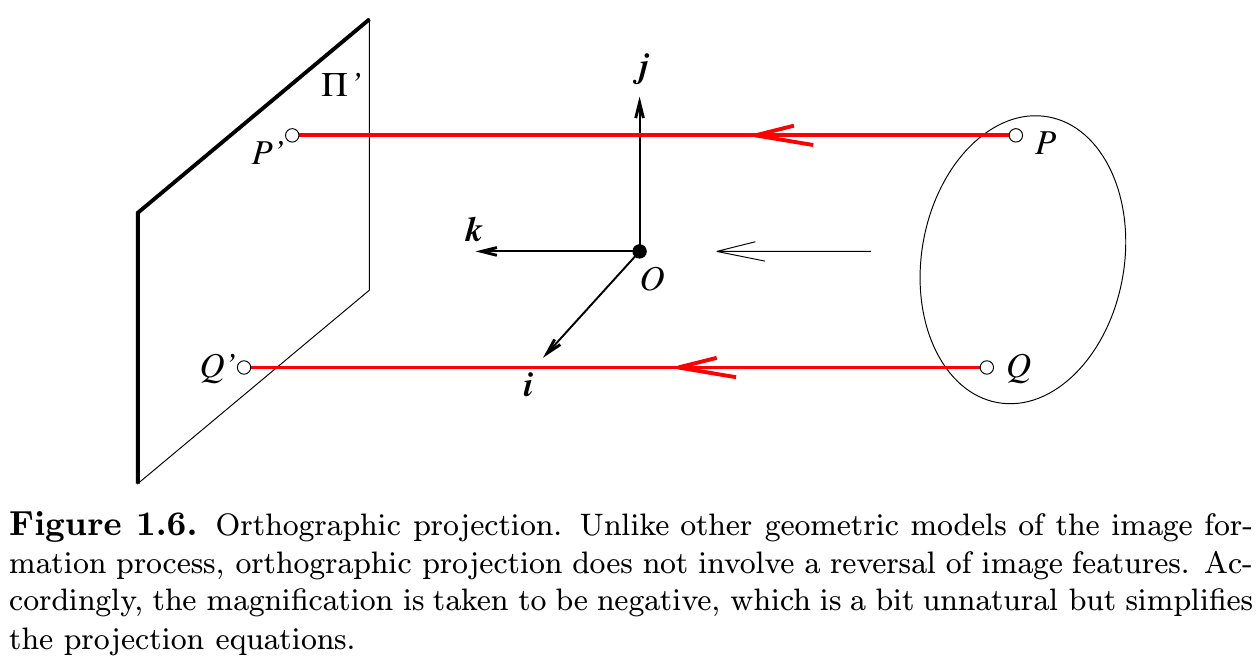
\includegraphics{img/orthographic_projection.png}}
\end{frame}}{\begin{frame}
  \frametitle{正交投影模型}
  
  \
  
  
  \begin{eqnarray*}
    x' & = & x\\
    y' & = & y
  \end{eqnarray*}
\end{frame}}{\begin{frame}
  \frametitle{球面投影}
  
  \
  
  {\hspace{3em}}\resizebox{0.8\columnwidth}{!}{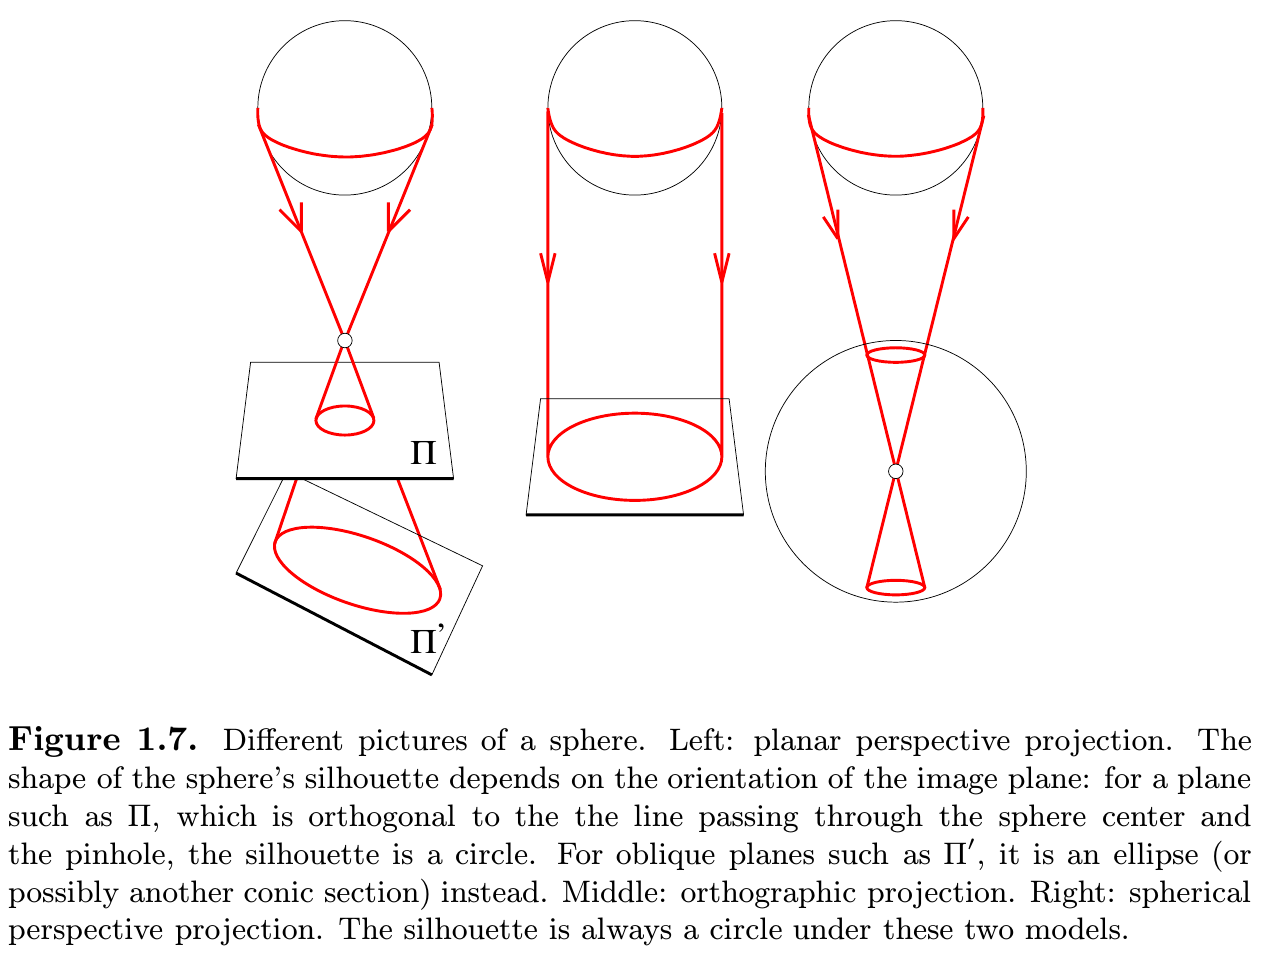
\includegraphics{img/sphere_pictures.png}}
\end{frame}}{\begin{frame}
  \frametitle{带镜头的相机}
  
  \
  
  {\hspace{4em}}\resizebox{0.7\columnwidth}{!}{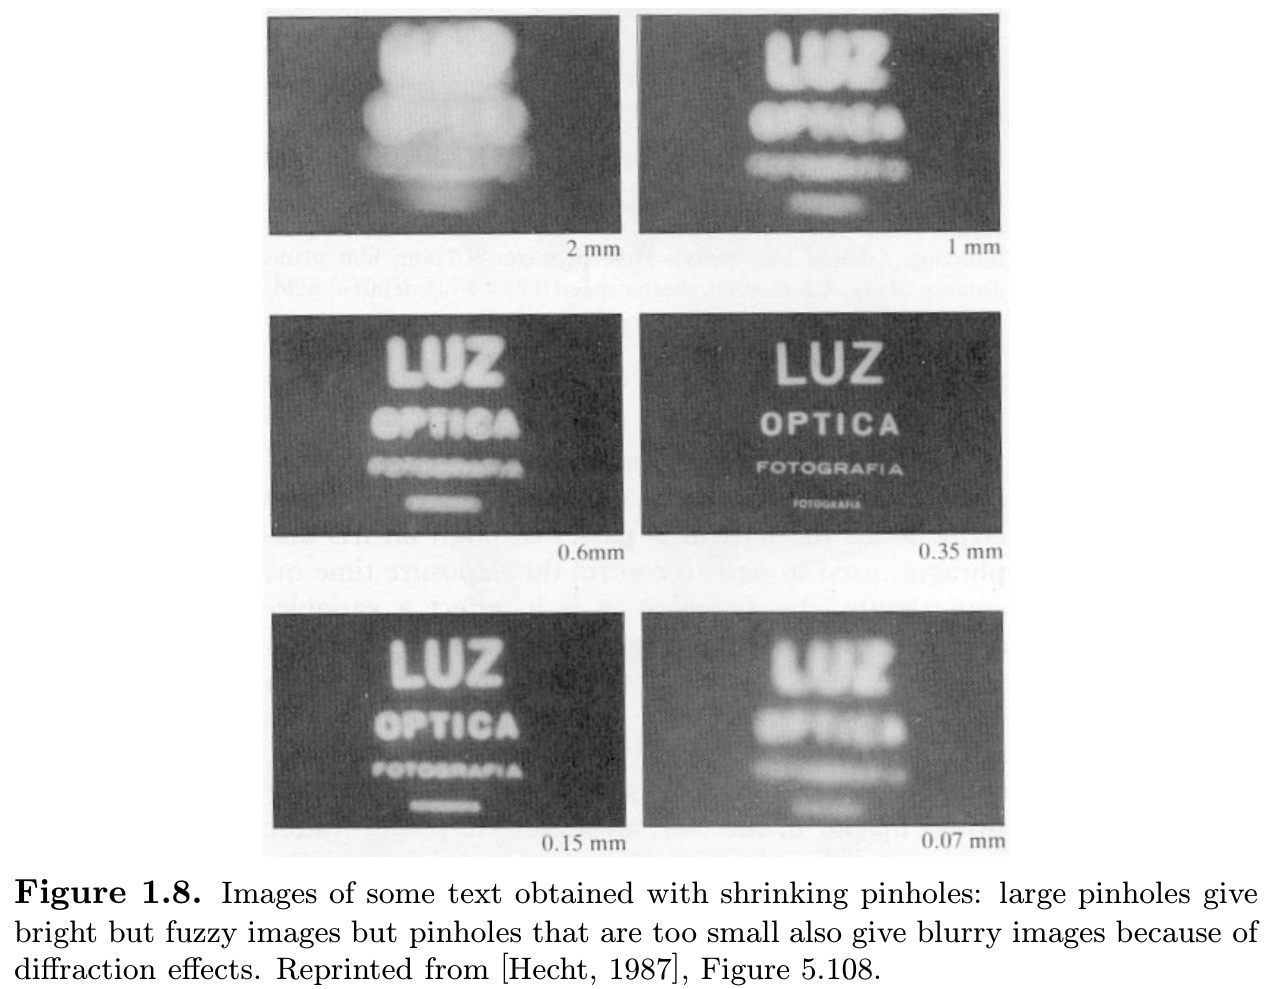
\includegraphics{img/pinhole_size.png}}
\end{frame}}{\begin{frame}
  \frametitle{折射与反射}
  
  \resizebox{1\columnwidth}{!}{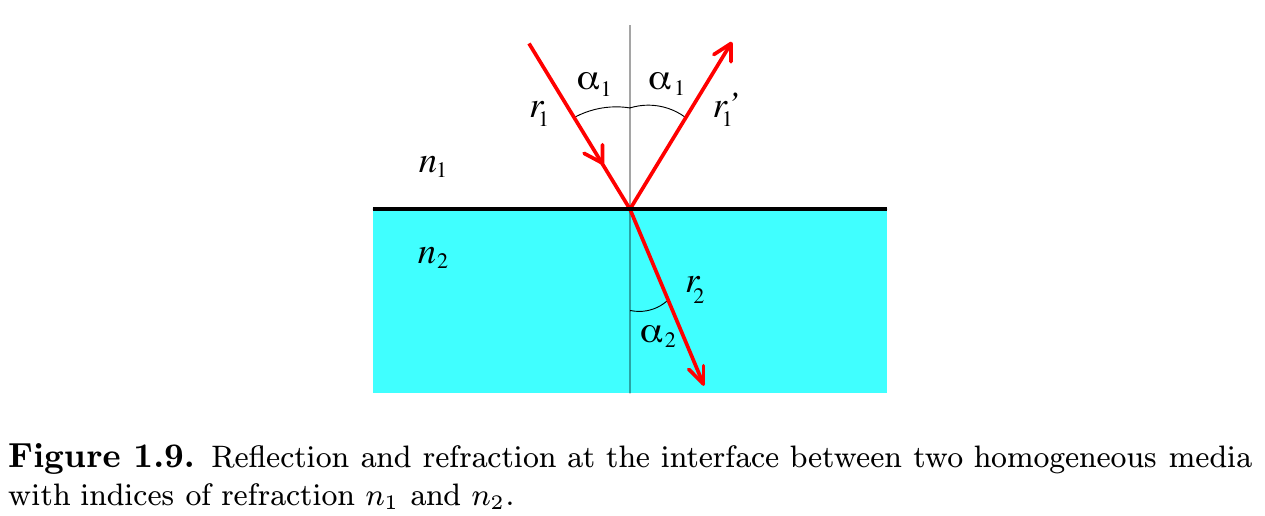
\includegraphics{img/reflection_refraction.png}}
  \begin{eqnarray*}
    n_1 \sin \alpha_1 & = & n_2 \sin \alpha_2
  \end{eqnarray*}
\end{frame}}{\begin{frame}
  \frametitle{近轴光学}
  
  \
  
  \resizebox{1\columnwidth}{!}{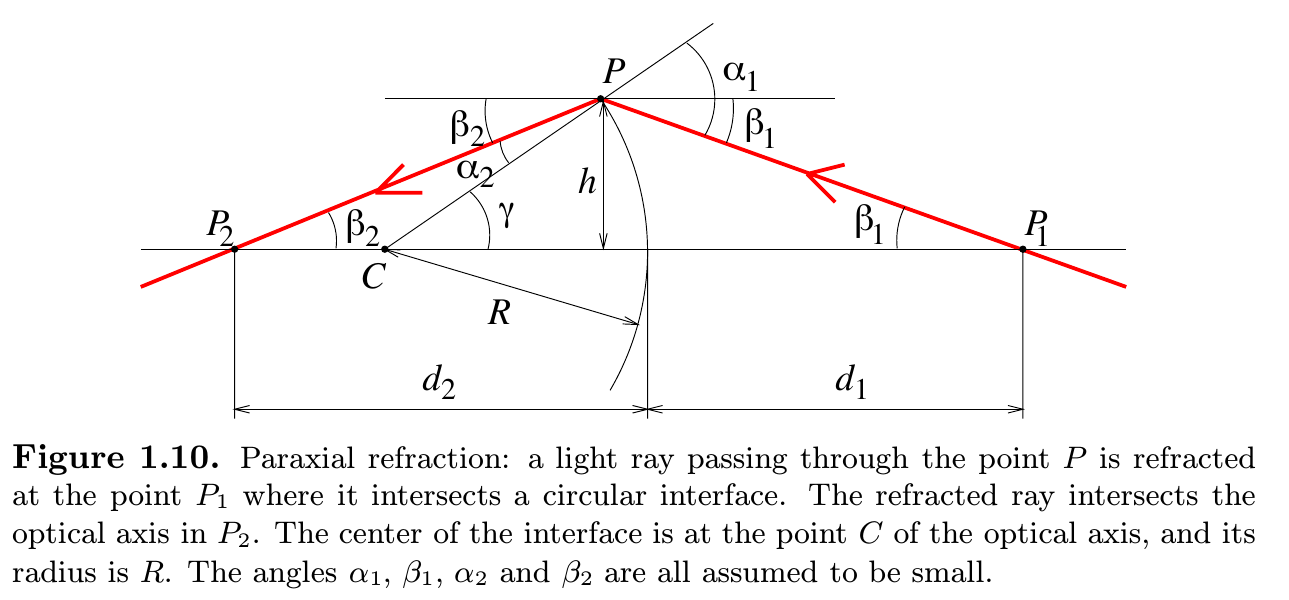
\includegraphics{img/paraxial_refraction.png}}
\end{frame}}{\begin{frame}
  \frametitle{}
  
  
  \begin{eqnarray*}
    \alpha_1 & = & \gamma + \beta_1\\
    & \approx & h \left( \frac{1}{R} + \frac{1}{d_1} \right)\\
    a_2 & = & \gamma - \beta_2\\
    & \approx & h \left( \frac{1}{R} - \frac{1}{d_2} \right)\\
    n_1 \alpha_1 & \approx & n_2 \alpha_2\\
    \frac{n_1}{d_1} + \frac{n_2}{d_2} & = & \frac{n_2 - n_1}{R}
  \end{eqnarray*}
  
\end{frame}}{\begin{frame}
  \frametitle{薄透镜}
  
  \resizebox{1\columnwidth}{!}{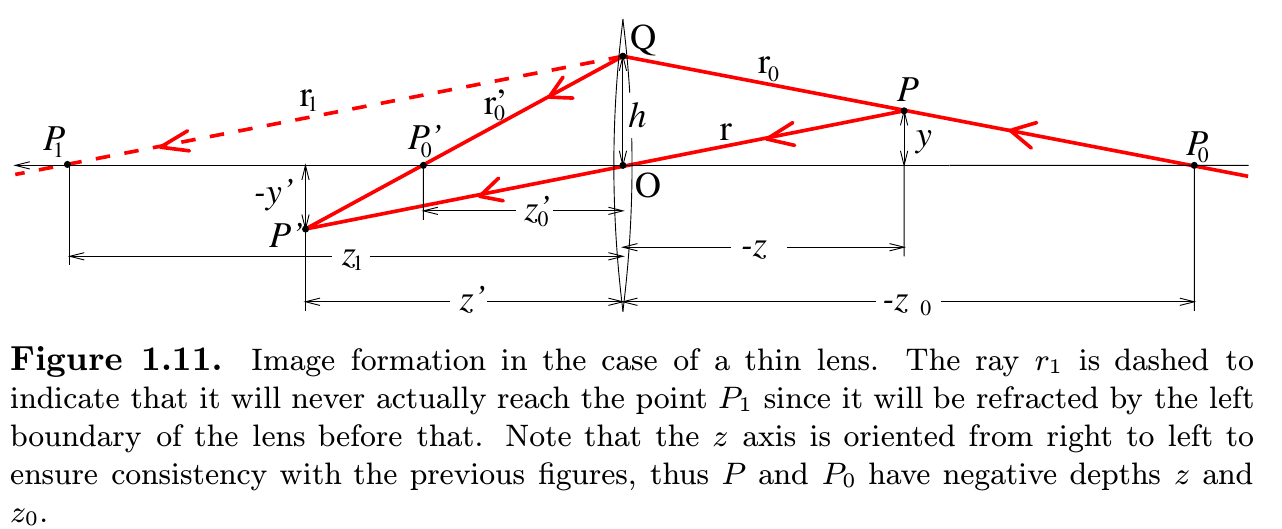
\includegraphics{img/thin_lens_imaging.png}}
\end{frame}}{\begin{frame}
  \frametitle{}
  \begin{eqnarray*}
    \frac{1}{R} + \frac{1}{- z_0} & = & n \left( \frac{1}{R} - \frac{1}{z_1}
    \right)\\
    n \left( \frac{1}{R} + \frac{1}{z_1} \right) & = & \frac{1}{R} +
    \frac{1}{z_0'}\\
    \frac{1}{z_0'} + \frac{1}{- z_0} & = & \frac{2 n - 2}{R}\\
    \frac{1}{z_0'} - \frac{1}{z_0} & = & \frac{1}{f} \hspace{4em} f =
    \frac{R}{2 n - 2}
  \end{eqnarray*}
\end{frame}}{\begin{frame}
  \frametitle{凸透镜成像}
  
  \
  
  {\hspace{4em}}\resizebox{0.7\columnwidth}{!}{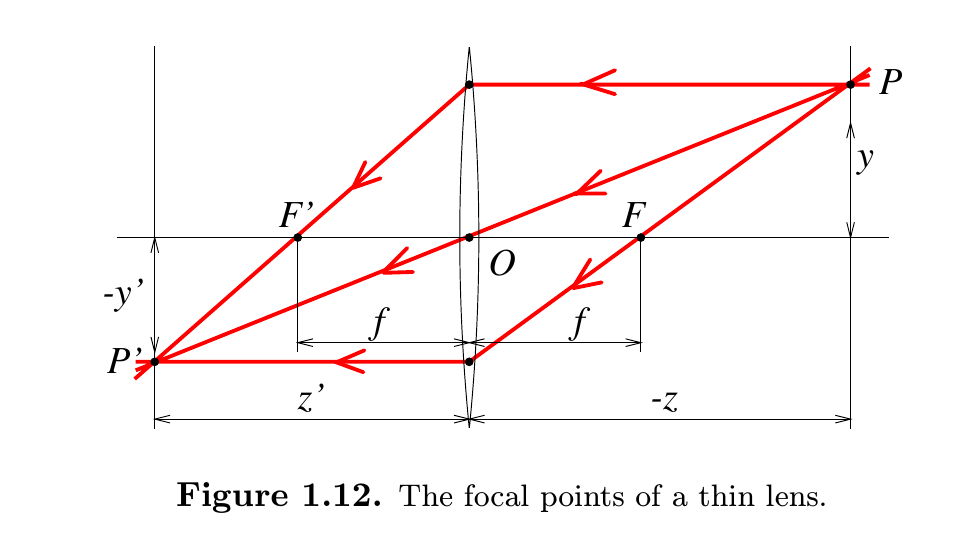
\includegraphics{img/thin_lens_focal_point.png}}
  \begin{eqnarray*}
    \frac{1}{z'} - \frac{1}{z} & = & \frac{1}{f}
  \end{eqnarray*}
\end{frame}}{\begin{frame}
  \frametitle{视场}
  
  \
  
  \resizebox{1\columnwidth}{!}{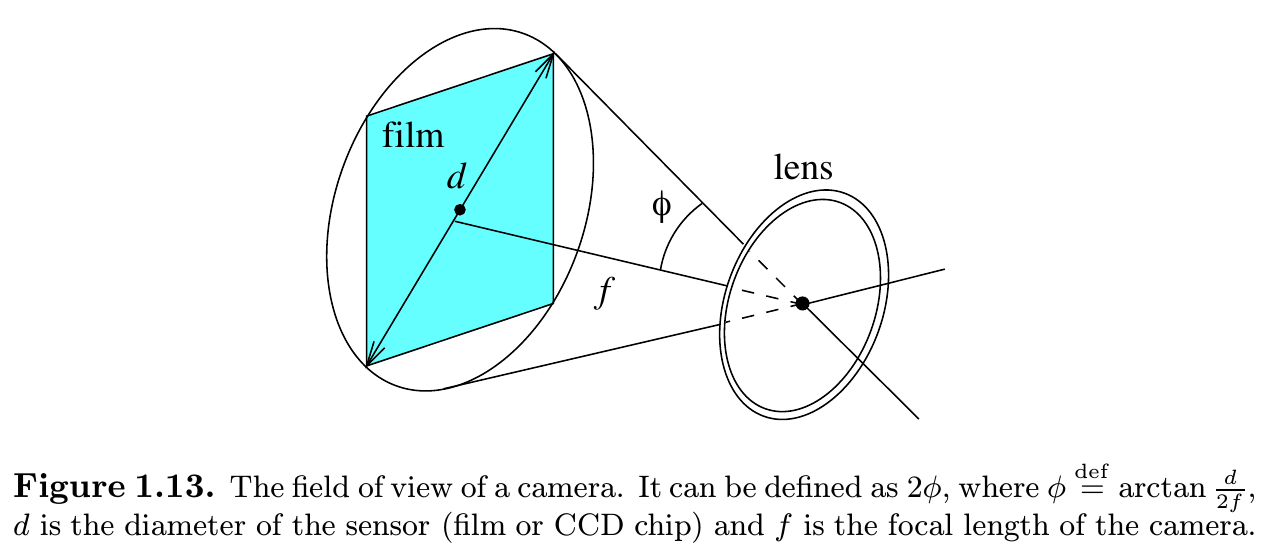
\includegraphics{img/field_of_view.png}}
\end{frame}}{\begin{frame}
  \frametitle{辐射度量学}
  
  \resizebox{1\columnwidth}{!}{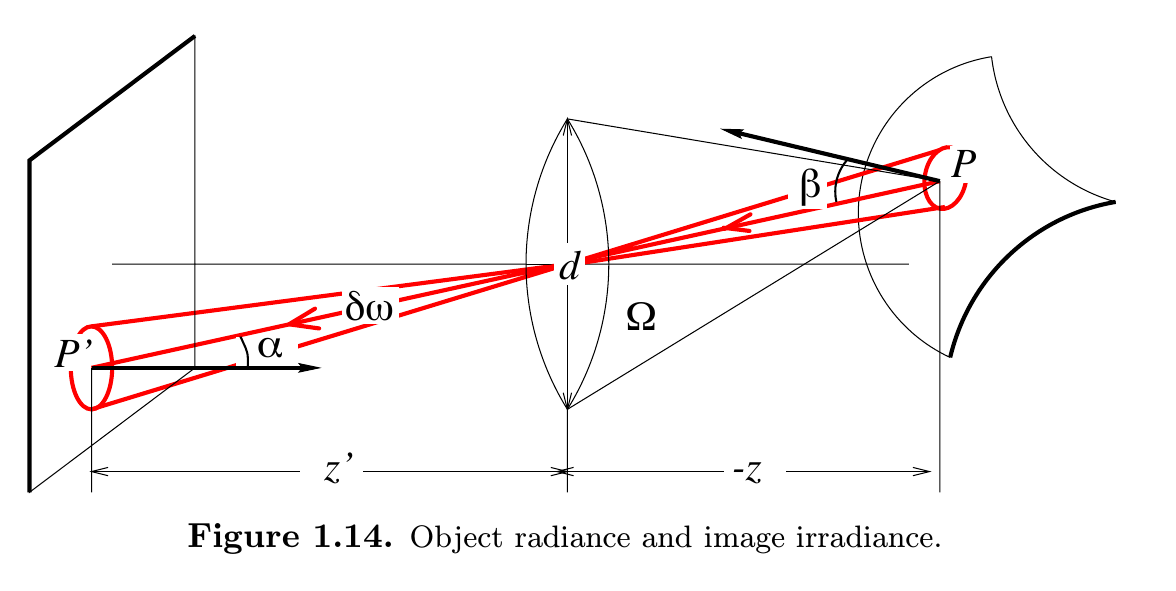
\includegraphics{img/radiance_irradiance.png}}
\end{frame}}{\begin{frame}
  \frametitle{}
  \begin{eqnarray*}
    \Omega & = & \frac{\pi d^2}{4} \cdummy \tmop{co} \alpha \cdummy \frac{1}{|
    \overrightarrow{\tmop{OP}} |^2}\\
    & = & \frac{\pi d^2}{4} \cdummy \frac{\cos^3 \alpha}{z^2}\\
    \delta P & = & L \Omega \delta A \nospace \cos \beta\\
    & = & \frac{\pi d^2}{4} \cdummy \frac{\cos^3 \alpha}{z^2} L \nospace \cos
    \beta \delta A \nospace\\
    E & = & \frac{\delta P}{\delta A'}\\
    & = & \frac{\pi d^2}{4} \cdummy \frac{\cos^3 \alpha}{z^2} L \nospace \cos
    \beta \frac{\delta A \nospace}{\delta A'}\\
    &  & 
  \end{eqnarray*}
\end{frame}}{\begin{frame}
  \frametitle{}
  \begin{eqnarray*}
    \frac{\delta A \nospace \cos \beta}{|  \overrightarrow{\tmop{OP}} |^2} & =
    & \frac{\delta A' \cos \alpha}{| \overrightarrow{\tmop{OP}'} |^2}\\
    \delta A \nospace \cos \beta \cdummy \frac{\cos^2 \alpha}{z} & = & \delta
    A' \cos^3 \alpha \cdummy \frac{\cos^2 \alpha}{z'}\\
    \frac{\delta A}{\delta A'} & = & \frac{\cos \alpha}{\cos \beta} \left(
    \frac{z}{z'} \right)^2\\
    E & = & \frac{\pi d^2}{4} \cdummy \frac{\cos^3 \alpha}{z^2} L \nospace
    \cos \beta \frac{\delta A \nospace}{\delta A'}\\
    & = & \frac{\pi}{4} \left( \frac{d}{{z'} } \right)^2 \nospace \cos^4
    \alpha L
  \end{eqnarray*}
\end{frame}}{\begin{frame}
  \frametitle{真实透镜}
  
  \resizebox{1\columnwidth}{!}{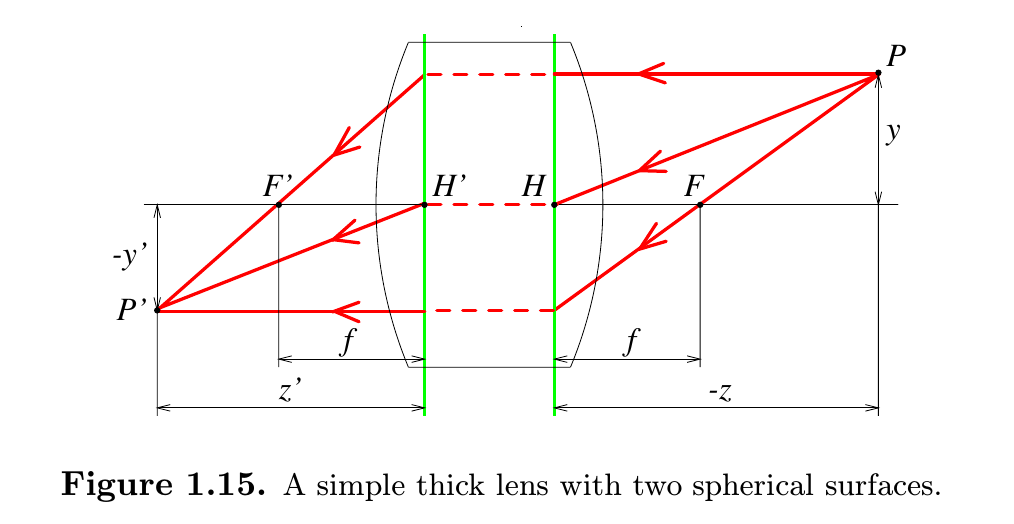
\includegraphics{img/thick_lens.png}}
\end{frame}}{\begin{frame}
  \frametitle{球面像差}
  
  \resizebox{1\columnwidth}{!}{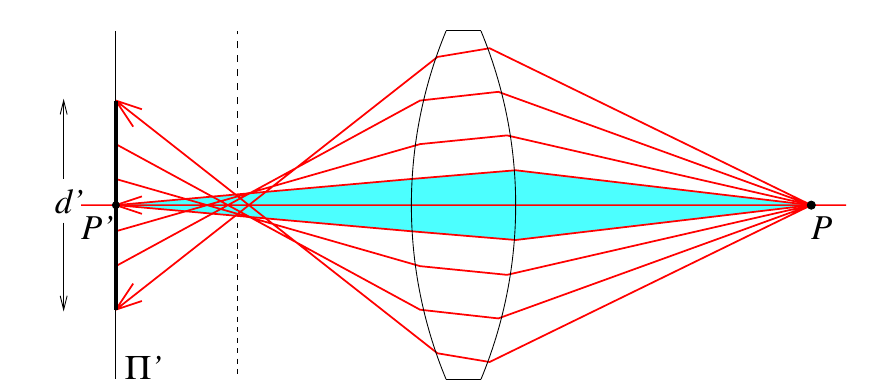
\includegraphics{img/spherical_aberration.png}}
  
  \ 
\end{frame}}{\begin{frame}
  \frametitle{畸变}
  
  \
  
  \resizebox{1\columnwidth}{!}{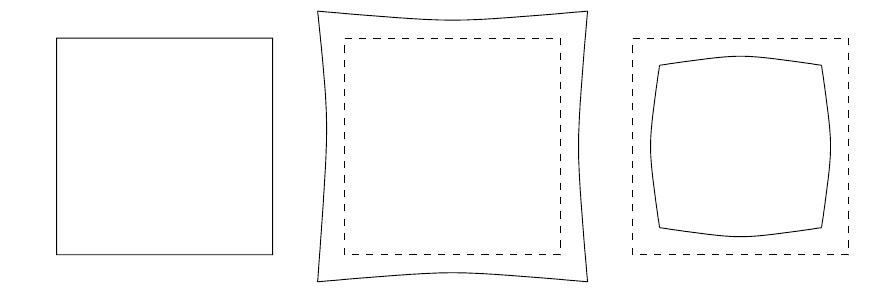
\includegraphics{img/distortion.png}}
\end{frame}}{\begin{frame}
  \frametitle{色像差}
  
  \
  
  \
  
  \resizebox{1\columnwidth}{!}{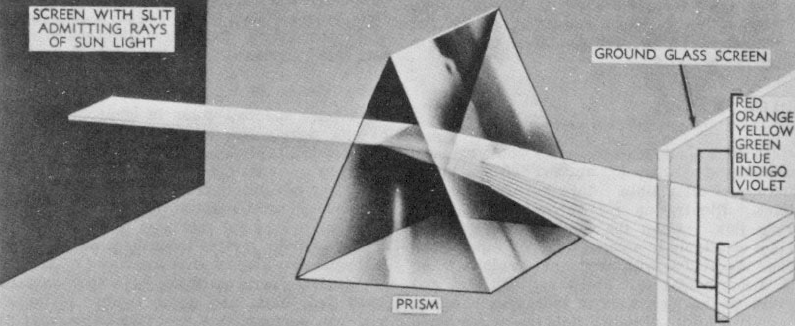
\includegraphics{img/chromatic_aberration.png}}
\end{frame}}{\begin{frame}
  \frametitle{透镜组}
  
  \resizebox{1\columnwidth}{!}{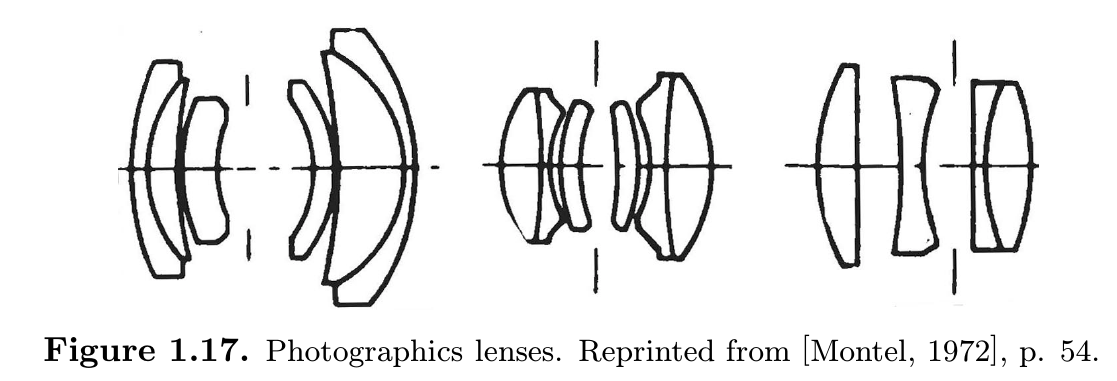
\includegraphics{img/photographics_lenses.png}}
\end{frame}}{\begin{frame}
  \frametitle{渐晕}
  
  \
  
  \resizebox{1\columnwidth}{!}{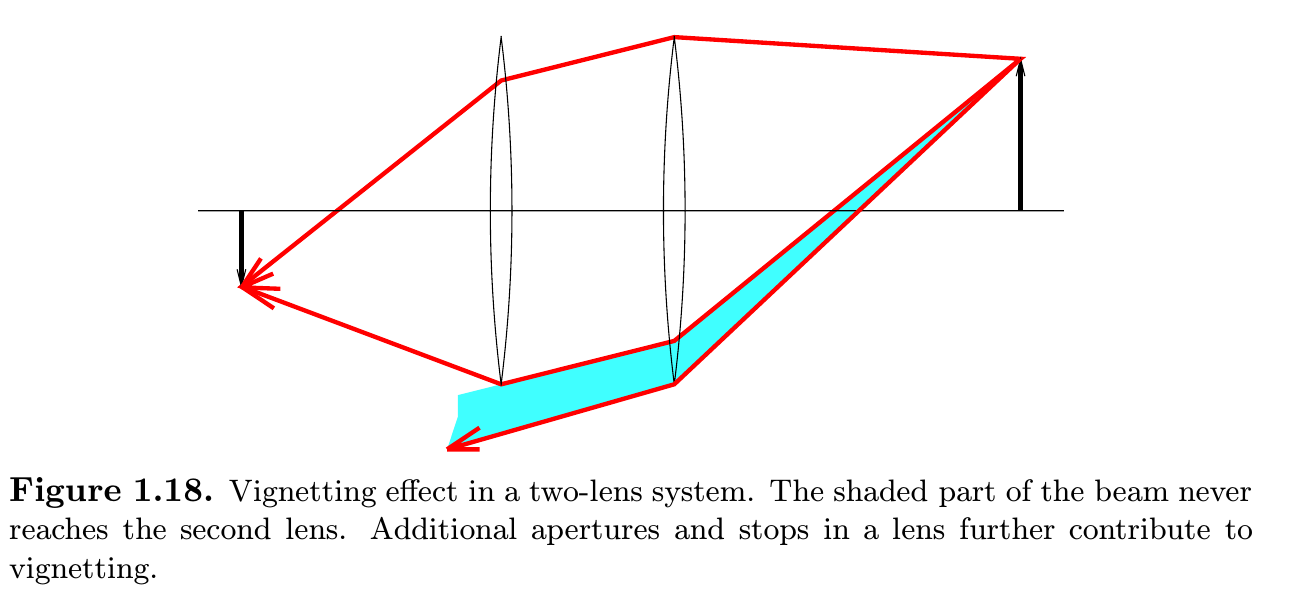
\includegraphics{img/vignetting_effect.png}}
\end{frame}}{\begin{frame}
  \frametitle{人眼}
  
  \
  
  \
  
  \resizebox{1\columnwidth}{!}{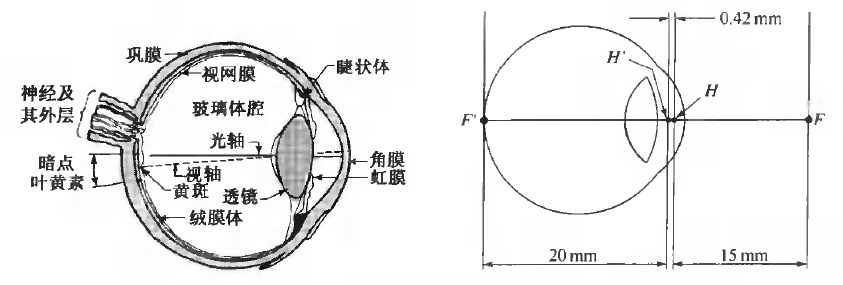
\includegraphics{img/human_eye.png}}
\end{frame}}{\begin{frame}
  \frametitle{{\tmstrong{视锥细胞响应曲线}}}
  
  {\hspace{3em}}\resizebox{0.8\columnwidth}{!}{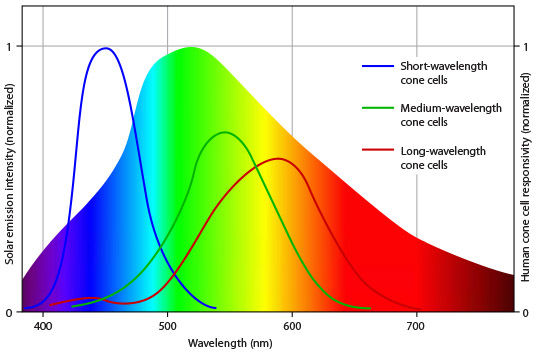
\includegraphics{img/cone_cell_response.png}}
  
  {\hspace{7em}}\href{http://weeklysciencequiz.blogspot.com}{http://weeklysciencequiz.blogspot.com}
\end{frame}}{\begin{frame}
  \frametitle{传感器}
  
  \
  
  \resizebox{1\columnwidth}{!}{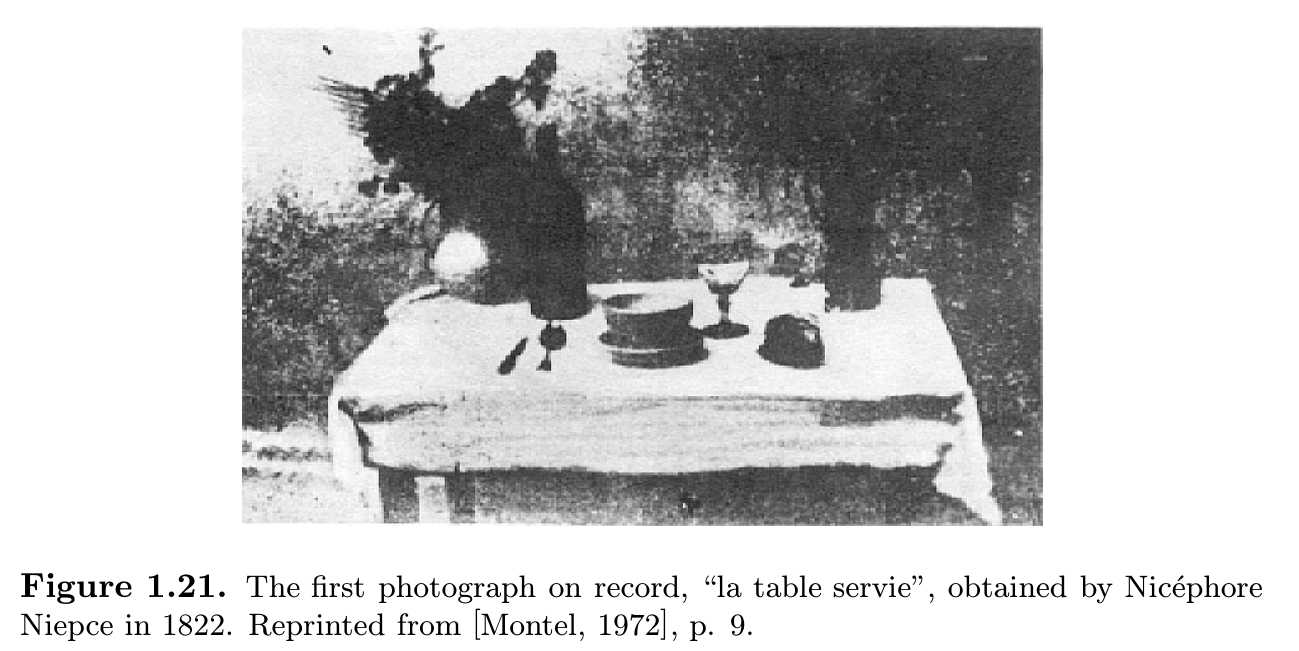
\includegraphics{img/first_photograph.png}}
\end{frame}}{\begin{frame}
  \frametitle{CCD}
  
  \
  
  {\hspace{8em}}\resizebox{0.5\columnwidth}{!}{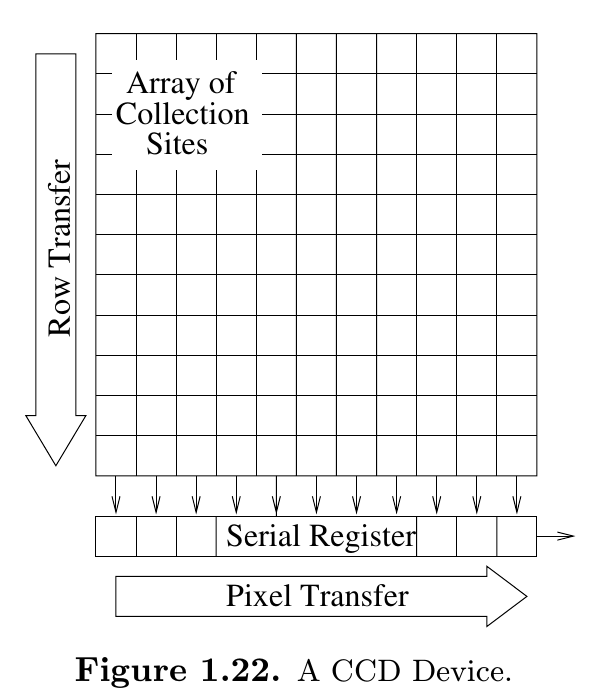
\includegraphics{img/ccd.png}}
\end{frame}}{\begin{frame}
  \frametitle{传感器模型}
  \begin{itemize}
    \item
    \begin{eqnarray*}
      I (r, c) & = & T \int_{\lambda} \int_{\tmmathbf{p} \in S (r, c)} E
      (\tmmathbf{p}, \lambda) R (\tmmathbf{p}) q (\lambda) \mathd \tmmathbf{p}
      \mathd \lambda
    \end{eqnarray*}
    \item
    \begin{eqnarray*}
      D (r, c) & = & \gamma (N_I (r, c) + N_{\tmop{DC}} (r, c) + N_B (,
      \tmop{rc}) + R (r, c)) + Q (, r, c)
    \end{eqnarray*}
    
  \end{itemize}
\end{frame}}}}}

\end{document}
